\section*{Part 3 [34 points]}

\begin{enumerate}
    \item \textbf{[17 points]} With your scheduling policy, run the entire workflow \textbf{\textcolor{red}{3 separate times}}. For each run, measure the execution time of each PARSEC job, as well as the latency outputs of memcached running with a steady client load of 30K QPS. For each PARSEC application, compute the mean and standard deviation of the execution time \footnote{You should only consider the runtime, excluding time spans during which the container is paused.} across three runs. Also compute the mean and standard deviation of the total time to complete all jobs. Fill in the table below. Finally, compute the SLO violation ratio for memcached for the three runs; the number of data points with 95th percentile latency $>$ 1ms, as a fraction of the total number of data points while the jobs are running.  

    \textbf{Answer:} % Put your solution here
    \begin{table}[ht]
        \centering
        \begin{tabular}{ |c|c|c|c|c|} 
            \hline
            job name & mean time [s] & std [s] \\ \hline \hline
            \coloredcell{blackscholes}    & 68.66 & 2.49 \\  \hline
            \coloredcell{canneal}         & 126 & 6.48 \\  \hline
            \coloredcell{dedup}           & 22.66 & 0.94 \\  \hline
            \coloredcell{ferret}          & 139.33 & 2.05 \\  \hline
            \coloredcell{freqmine}        & 124.00 & 0.82 \\  \hline
            \coloredcell{radix}           & 86.00 & 2.16 \\  \hline
            \coloredcell{vips}            & 69.66 & 1.70 \\  \hline
            total time      & 143.66 & 1.25 \\ \hline
        \end{tabular}
    \end{table}

    \begin{itemize}
        \item Generally, the memcached p95 latency is around 0.5ms. The SLO violation ratio is 0.0 for all runs, since the number of data points with 95th percentile latency $>$ 1ms is 0 for all runs. 
    \end{itemize}
    
    Create 3 bar plots (one for each run) of memcached p95 latency (y-axis) over time (x-axis) with annotations showing when each PARSEC job started and ended, also indicating the machine they are running on. Using the augmented version of mcperf, you get two additional columns in the output: \texttt{ts\_start} and \texttt{ts\_end}. Use them to determine the width of each bar while the height should represent the p95 latency. Align the $x$ axis so that $x=0$ coincides with the starting time of the first container. Use  the colors proposed in this template (you can find them in \texttt{main.tex}). For example, use the \colored{vips} color to annotate when vips started.

    \textbf{Plots:} % Put your plots here

    \begin{figure}[htbp]
        \centering
        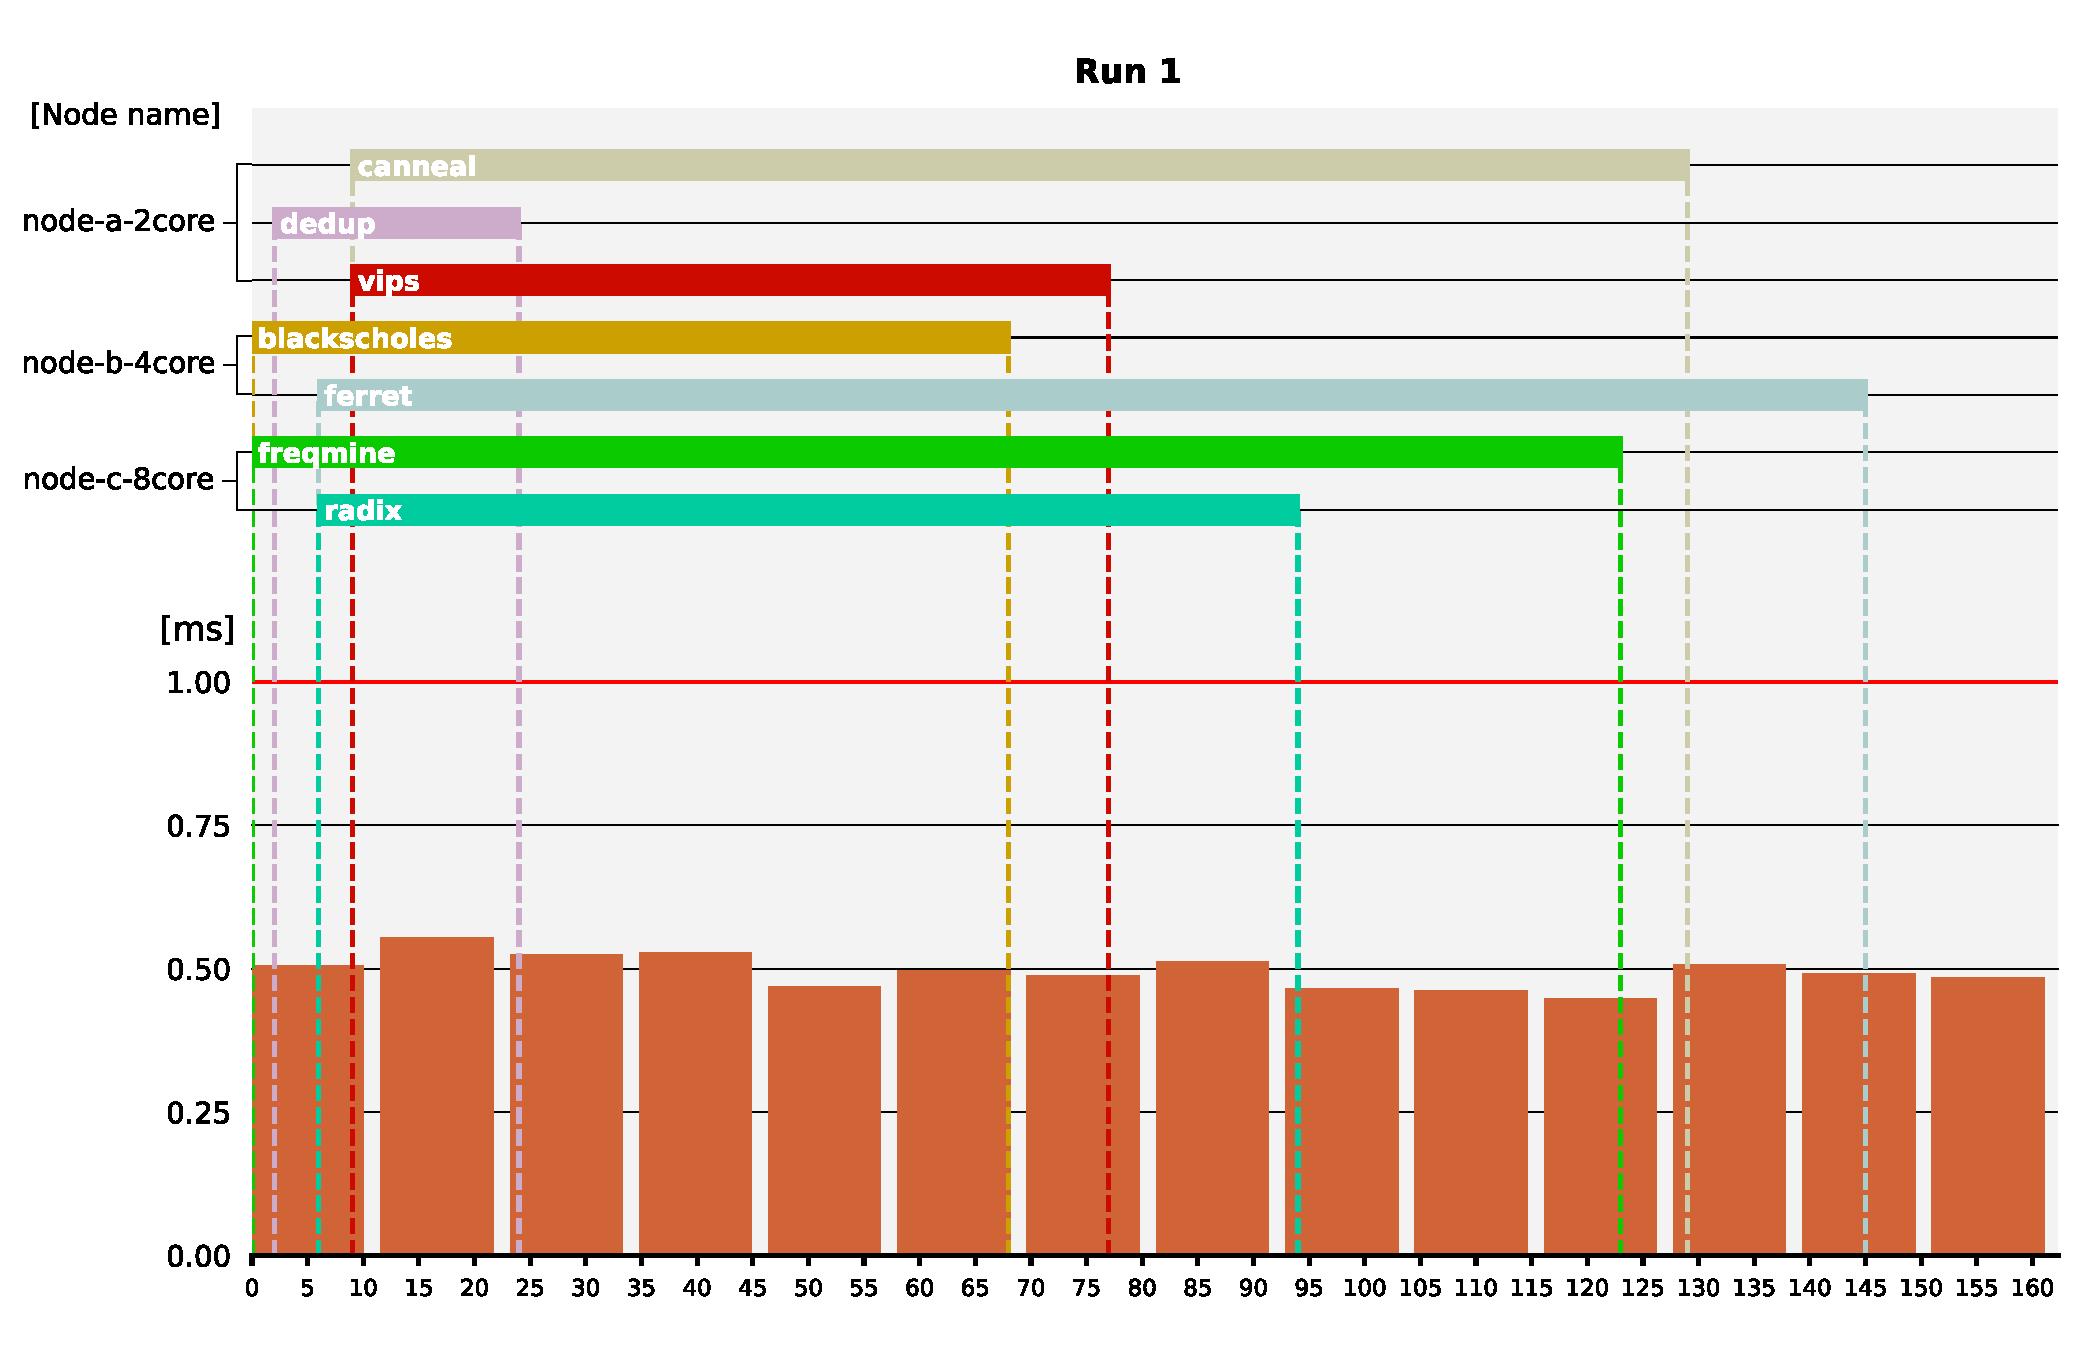
\includegraphics[width=.9\linewidth]{figures/part3/plot3_run_1}
        \caption{Run 1}
        \label{fig:plot3_run_1}
    \end{figure}

    \begin{figure}[htbp]
        \centering
        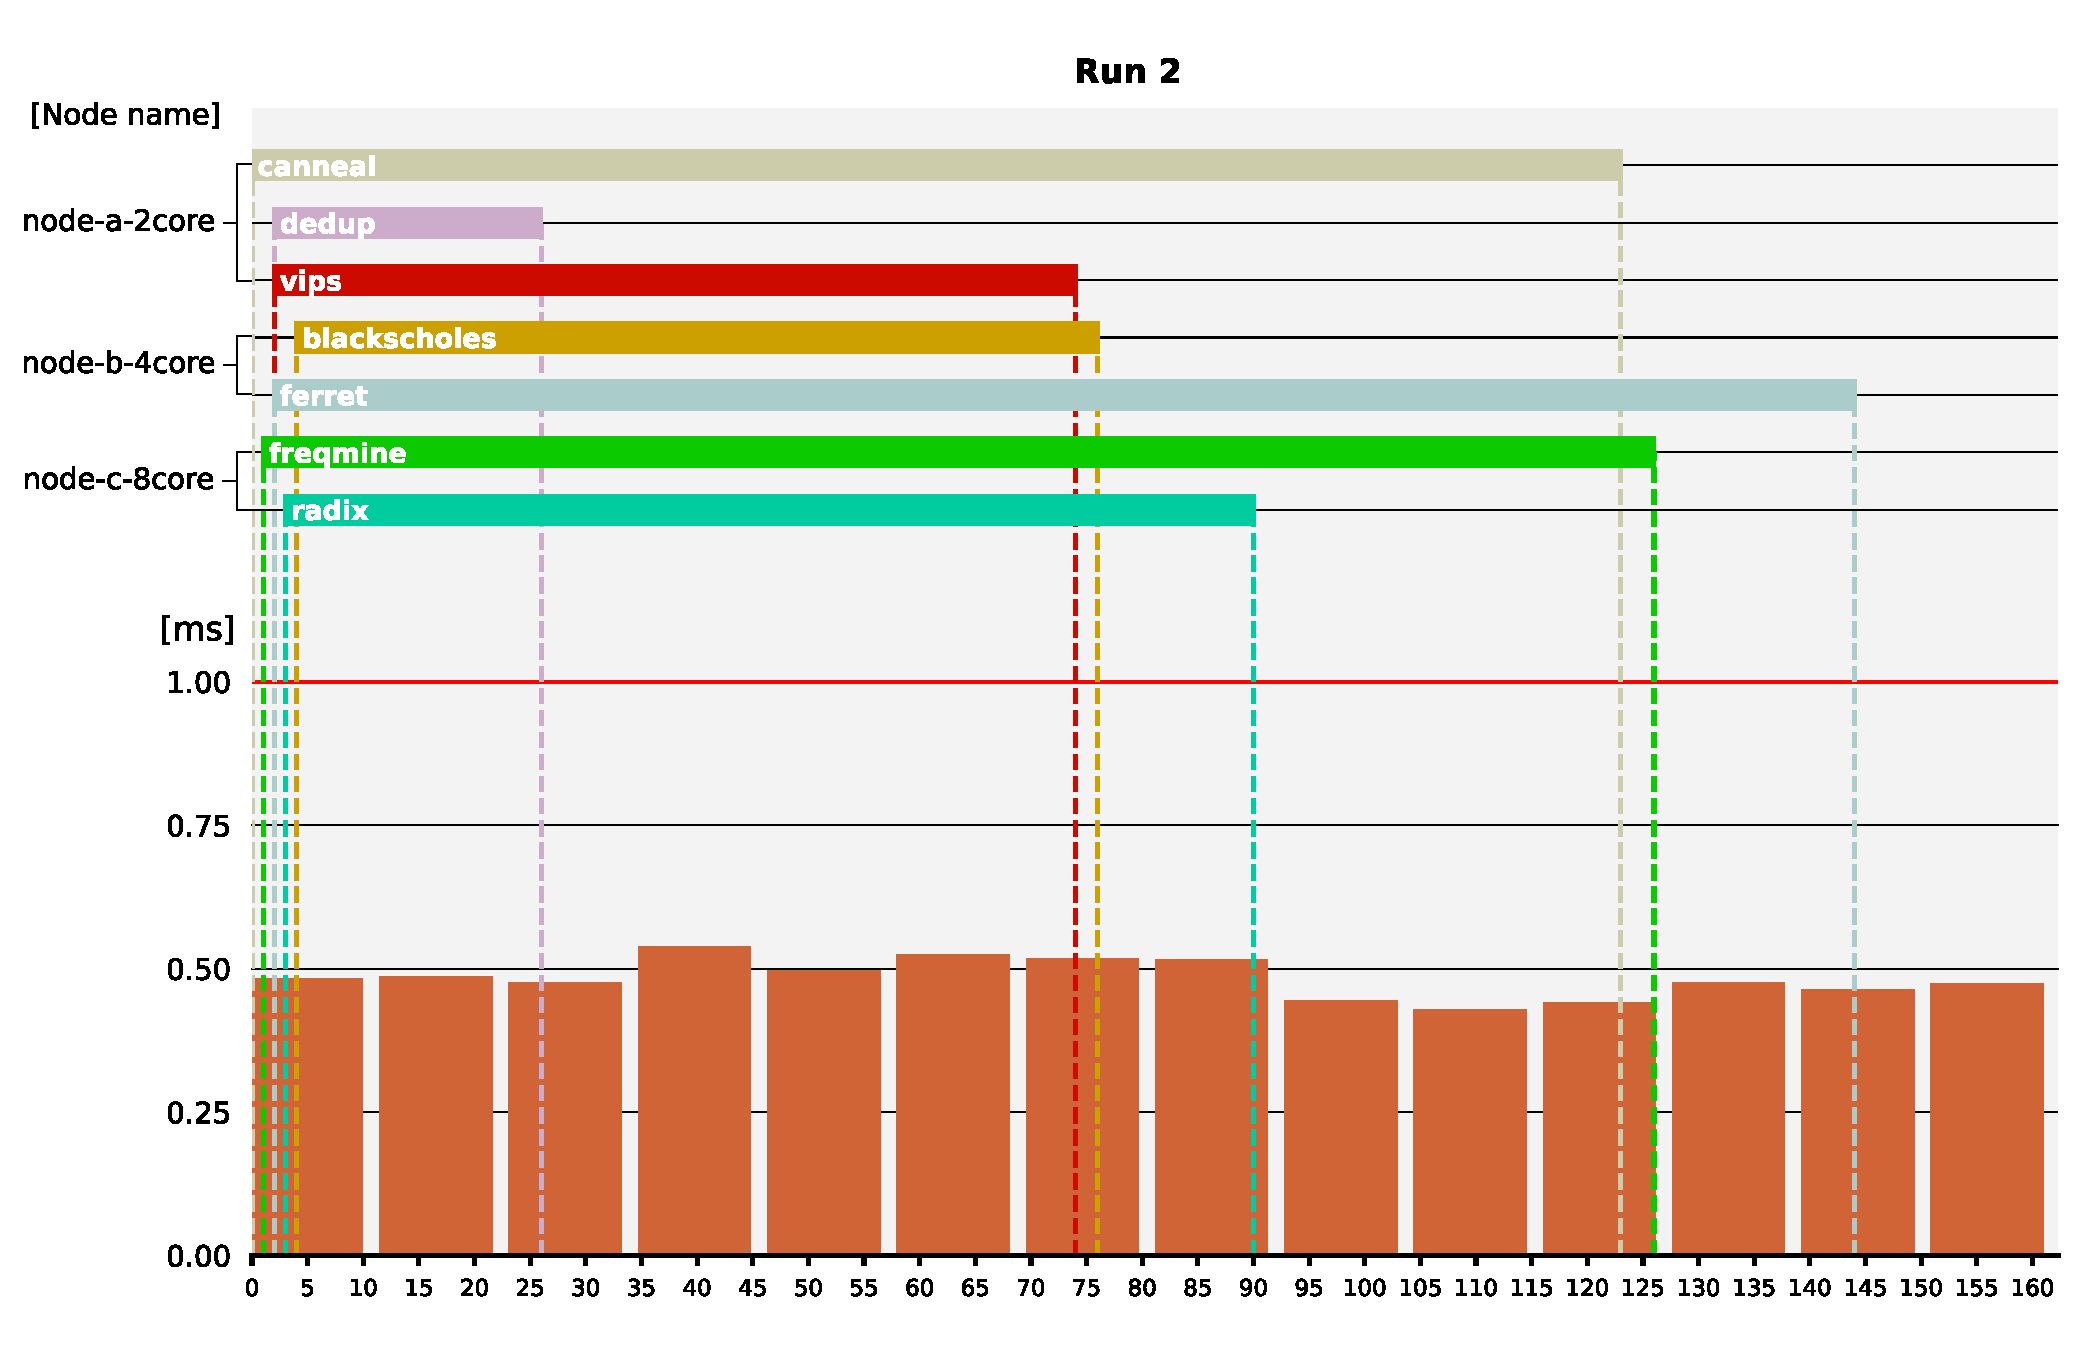
\includegraphics[width=.9\linewidth]{figures/part3/plot3_run_2}
        \caption{Run 2}
        \label{fig:plot3_run_2}
    \end{figure}

    \begin{figure}[htbp]
        \centering
        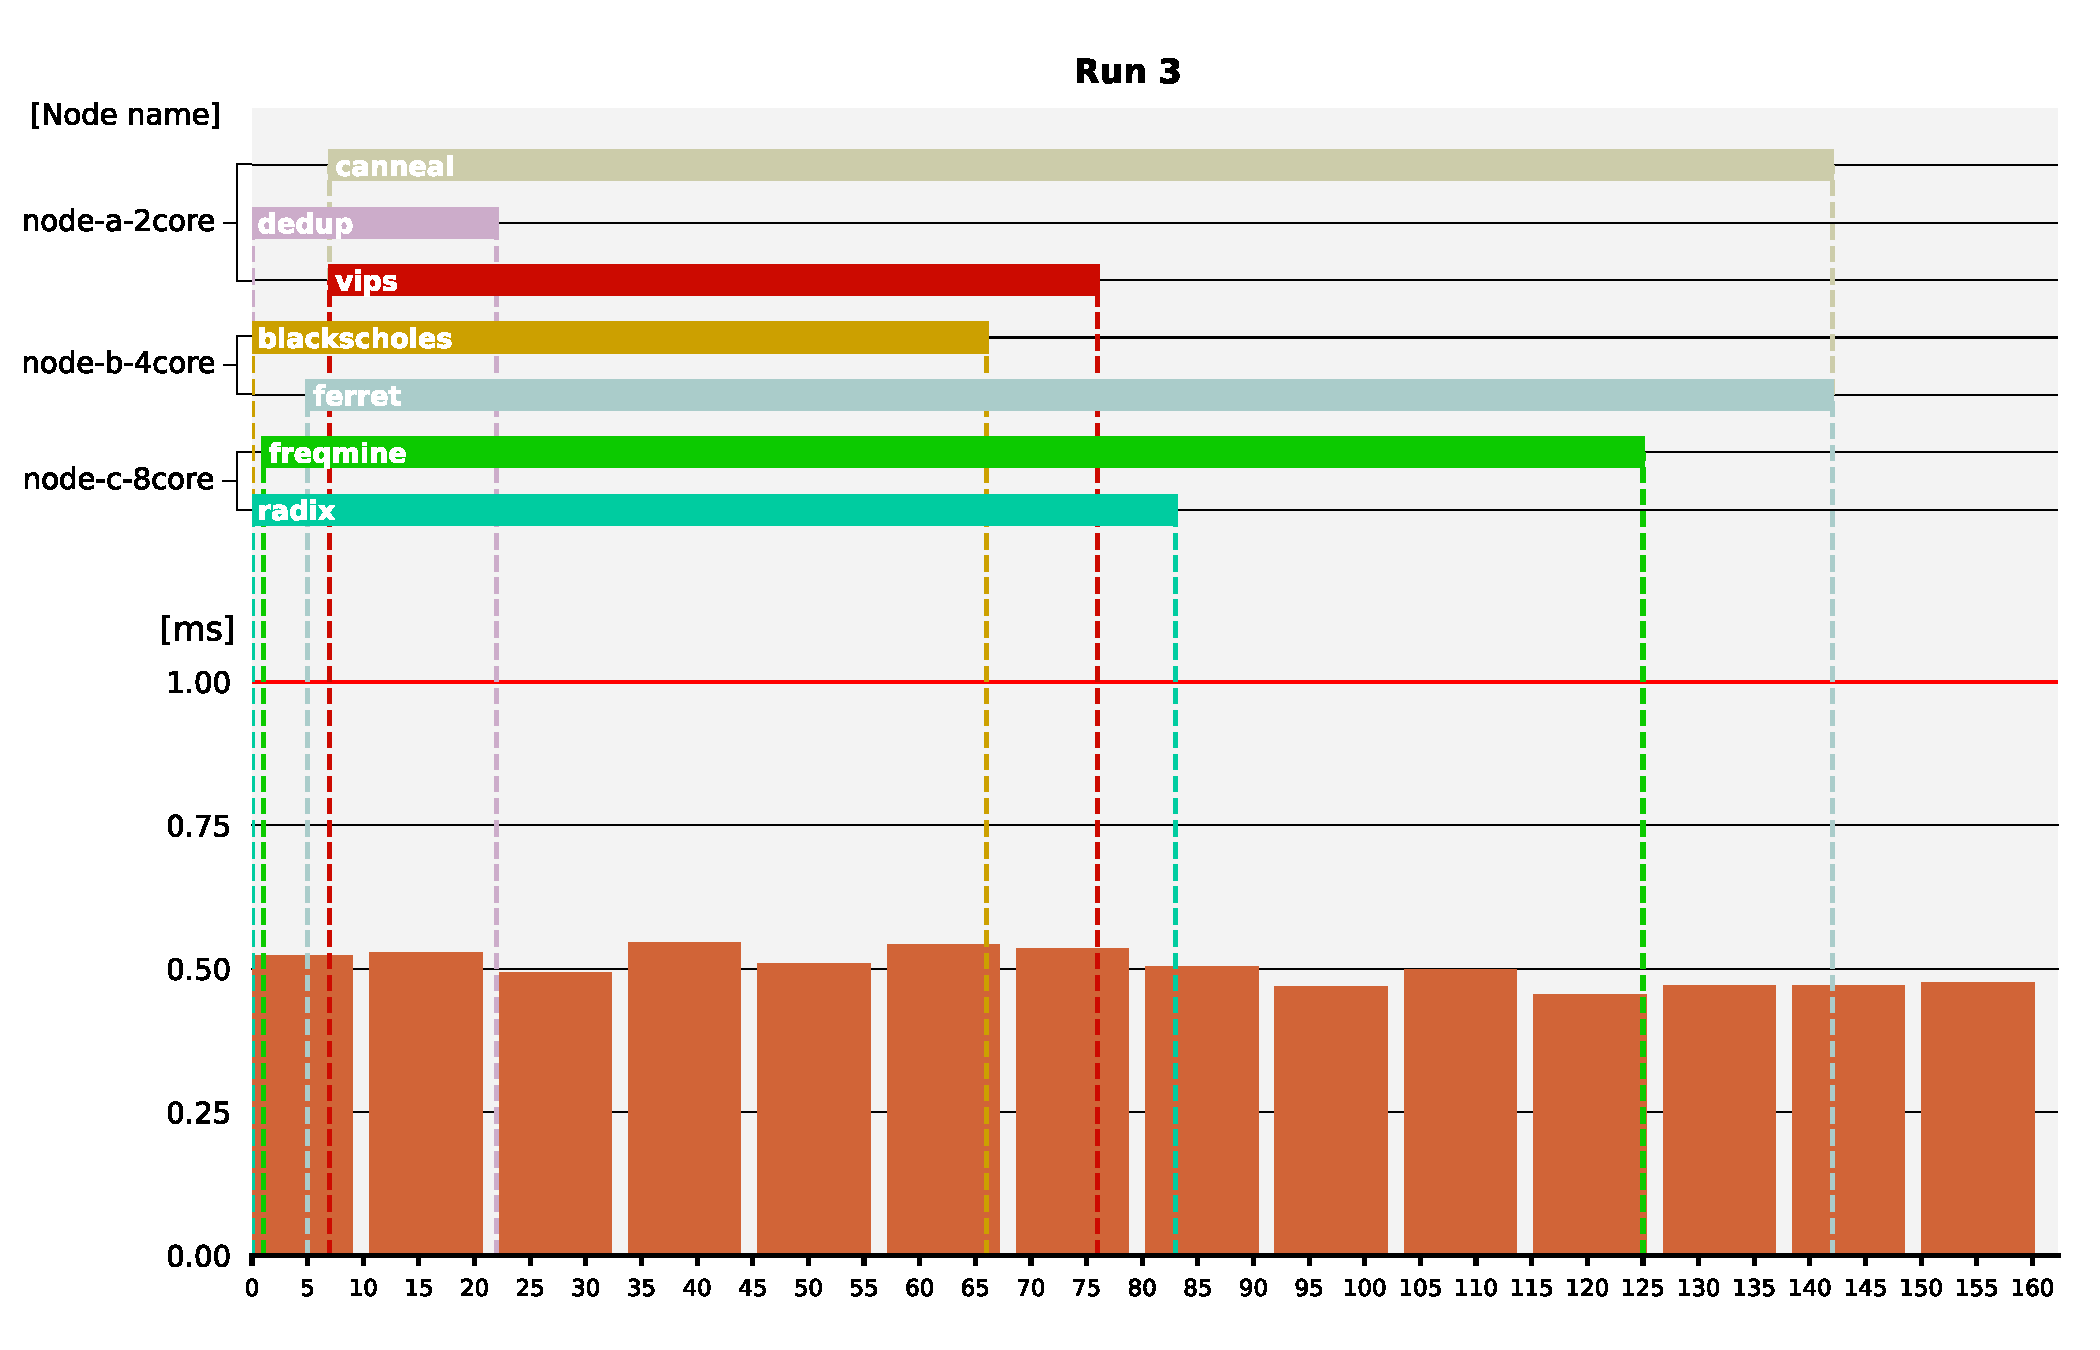
\includegraphics[width=.9\linewidth]{figures/part3/plot3_run_3}
        \caption{Run 3}
        \label{fig:plot3_run_3}
    \end{figure}

    \FloatBarrier
    
    \item \textbf{[17 points]} Describe and justify the “optimal” scheduling policy you have designed. 
    
    \begin{itemize}
        \item Which node does memcached run on? Why?

        \textbf{Answer:} % Put your solution here
        Memcached is running on node-c-8core with its CPU affinity set to CPU 0. We took into account several factors while deciding the node for memcached.

        Firstly, memcached does not require much CPU and memory while operating at a constant 30K QPS. Testing it, we found out that it needs just 0.5 CPU and 32MB memory to run smoothly.
        
        Secondly, after consulting the documentation, we discovered that the e2-standard-8 machine, despite having the highest number of cores, has weaker CPUs compared to the other machines. Therefore, we decided to reserve the faster machines for Parsec jobs.
        
        We requested at least 0.5 CPU and 32 MB memory for memcached and limited  to maximum 0.75 CPU and 64 MB respectively using Kubernetes. This configuration prevented other Parsec jobs running on the same machine and same core from using all the CPUs and memory which would have resulted in a higher latency for memcached.

        \item Which node does each of the 7 PARSEC jobs run on? Why?

        \textbf{Answer:}
        \begin{itemize}
            \item \colored{blackscholes}: % Put your solution here
            Node-b, because it performs good with four threads and node-b has four cores, providing a good environment for it to run efficiently. Assigning it less core while ferret is running on the same node would have resulted in a higher execution time of blackscholes and as a consequence a higher ferret execution time.
            
            \item \colored{canneal}: % Put your solution here
            Node-a, as it does not demand many resources but needs two cores to minimize its execution time.

            \item \colored{dedup}: % Put your solution here
            Node-a, despite being a very demanding job, it is quick to run and one core on Node-a can accommodate it.
            
            \item \colored{ferret}: % Put your solution here 
            Node-b, as it's high in CPU demand and scales well with the available cores. It is one of the most demanding jobs CPU and memory wise, we assigned also blackscholes in this node because it is not a very demanding job and they fit togheter.

            \item \colored{freqmine}: % Put your solution here
            Node-c, as it scales well with the number of cores and the eight cores of node-c helps minimize its execution time. It is the longest job to run, so we assigned it to the node with the most cores. 
            
            \item \colored{radix}: % Put your solution here
            Node-c, as it has the least resource requirements, and just one of the low performing cores in node-c is sufficient for it. Being very low demanding do not interfere much with freqmine neither interfere at all with memcached.

            \item \colored{vips}: % Put your solution here
            Node-a, because it requires high memory transfer speed which node-a provides being the best spec machine amongst all.
            
        \end{itemize}

        Further explanation on our motivations is given in the section regarding design choices at the end of Part 3.

        \item Which jobs run concurrently / are colocated? Why?

        \textbf{Answer:} % Put your solution here
        On node-a, canneal, dedup, and vips are run concurrently because it minimizes the total execution time compared to running them sequentially.
        
        On node-b, blackscholes and ferret are run concurrently. Even though ferret's execution time increases by 20\% when colocated with blackscholes, the total time for running both is less than running them separately.
        
        On node-c, freqmine and radix are run concurrently. Radix shares the core with the memcached server because it has low resource needs and doesn't interfere with the server's performance.

        \item In which order did you run 7 PARSEC jobs? Why?
    
        \textbf{Order}: % Sort them 
        \colored{blackscholes}, \colored{canneal}, \colored{dedup}, \colored{ferret}, \colored{freqmine}, \colored{radix}, \colored{vips}
    
    
        \textbf{Why}: % Put your solution here
        All the jobs are started \textbf{concurrently} on the three nodes, hence there is no order in which they are started.

        \item How many threads have you used for each of the 7 PARSEC jobs? Why?
    
        \textbf{Answer:}
    
        \begin{itemize}
            \item \colored{blackscholes}: % Put your solution here
            Four threads because it performs better with four threads and 4 cores. Assigning it less threads would have increased its execution time exceeding the achieved runtime. Using two cores has been tested but it is not as efficient as using four cores because it takes long to complete and interfere longer with ferret that is a demanding job running on the same node.

            \item \colored{canneal}: % Put your solution here
            Two threads as it is run on node-a which has two cores, and this minimizes its execution time. Using more thread is not beneficial as it doesn't scale well with more than two thread.

            \item \colored{dedup}: % Put your solution here
            One thread, as it runs on one core of node-a and completes quickly. Moreover it doesn't scale well with more threads. Just one core was assigned also to interfere less with canneal that is running on the same node.

            \item \colored{ferret}: % Put your solution here 
            Four threads, as it is run on node-b, which has four cores, and it scales well with more cores.

            \item \colored{freqmine}: % Put your solution here
            Eight threads because it is run on node-c which has eight cores and it scales well with the number of cores. Using four threads would have increased its execution time significantly.

            \item \colored{radix}: % Put your solution here
            One thread because it has low resource requirements and shares a core with the memcached server on node-c. It is actually run with just 0.1 CPU and a hard limit on 0.25 to not interfere with the memcached server. It does not interfere also with freqmine that is a demanding job running on the same node.

            \item \colored{vips}: % Put your solution here
            One thread because it is quick to run and it can share the core only with canneal, using two cores would mean share the core with three process concurrently. It is assigned in the other core respect to dedup, so they do not interfere with each other ends quickly and leave the resources to canneal.
        \end{itemize}



        \item Which files did you modify or add and in what way? Which Kubernetes features did you use?
    
        \textbf{Answer:} % Put your solution here
        We revised seven YAML configuration files corresponding to the seven PARSEC jobs. The modifications involved setting the number of threads each job should use, defining the CPU affinity via the \texttt{taskset} command and the \texttt{nodeSelector} property to specify on which node each job should run.
        
        Additionally, the YAML configuration file for the memcached server was adjusted to specify the resource request using Kubernetes feature \texttt{Resources} using both \texttt{Request} and \texttt{limit} to set how much CPU and memory a job is assured to use and the maximum it can use respectively.
        
        A Python script was developed to automate the process of job creation, memcached server setup, and the implementation of the scheduling mechanism. Find below the output of the help command of this script which describes the different functionalities it provides.

        % TODO: Maybe we can include the output of the help command as it is really well done

        \begin{verbatim}
python3 main.py --help
usage: main [-h] {create,status,start,stop,destroy,ssh,test,time} ...

Command line interface for cluster operations

positional arguments:
{create,status,start,stop,destroy,ssh,test,time}
    create              create cluster
    status              get status
    start               start service
    stop                stop service
    destroy             destroy cluster
    ssh                 ssh to a node
    test                test a scheduler
    time                analyze results

optional arguments:
-h, --help            show this help message and exit
        \end{verbatim}
        
        \vspace{1cm}

        \item Describe the design choices, ideas and trade-offs you took into account while creating your scheduler (if not already mentioned above):

        \textbf{Answer:} % Put your solution here
        The main design consideration for the scheduler was to minimize total execution time of all jobs, while not interfering much with the memcached execution. This was achieved by:
        \begin{itemize}
            \item Co-locating jobs that are compatible in terms of resource usage. For instance, ferret and blackscholes are run together on node-b, while canneal, dedup, and vips are colocate on node-a.
            \item Matching jobs with the right nodes based on their resource demands and the node's capabilities. For example, vips is put on node-a because it requires high memory transfer speed.
            \item Running jobs concurrently on each node instead of sequentially to minimize total execution time.
            \item Adjusting the number of threads each job uses according to the number of cores in each node and the individual job's performance under various thread counts. For instance, blackscholes runs with four threads on node-b because it performs better under these conditions, while freqmine uses all eight cores of node-c because it scales well with the number of cores.

        \end{itemize}

        The major trade-off in this scheduler design is slowing down the individual execution time of each job to minimize the total execution time. For example, the execution time of ferret increases by about 20\% when run together with blackscholes on node-b, but the total execution time of both jobs is less when run together compared to running them consecutively.

        Another trade-off is the choice to limit the number of cores/threads some jobs can use despite their ability to scale well with more cores. This decision is made to ensure other processes or jobs on the same node are not negatively affected. For example, radix, despite scaling the best with the number of cores, is limited to use only 0.25 core on node-c to avoid interfering with memcached, it is still very fast to complete and it would be a waste of CPU power to assign to it more CPUs. Similarly, vips, despite scaling well, is limited to use only one core on node-a to not compete with three jobs concurrently, also it is faster than canneal to complete and therefore canneal has been assigned two cores to complete faster.

        The design of the scheduler involves a delicate balance of maximizing the utilization of available resources, managing co-locations to minimize total execution time, and respecting the specific needs and characteristics of each job. These decisions have been taken looking at the characteristics of each job and the resources available on each node, and by running experiments to determine the best number of threads for each job. We took into account also the scalability and resource demand of each jobs tested on part 2.
        
        Looking at the documentation we realize that the most powerful CPU are in node-a, following node-b and node-c so we run every job alone in every machine with various number of threads and core to find how much time each jobs takes on each configuration to be able later with all the information to decide better where and how schedule the jobs. The results of this experiment can be found in \autoref{tab:my-table}

        %TODO: include the table with the times Lorenzo did

        \begin{table}[!htp]\centering
            \caption{Runtime (s) of PARSEC jobs on various configurations} \label{tab:my-table}
            \scriptsize
           
            \begin{tabular}{ccccc}\toprule
            \multicolumn{4}{c}{\textbf{Blackscholes}} \\
            \midrule
            Number of cores &Runtime in node-a &Runtime in node-b &Runtime in node-c \\
            \midrule
            1 &01:04 &01:33 &02:09 \\
            2 &00:37 &01:02 &01:16 \\
            4 & &00:49 &00:49 \\
            8 & & &00:38 \\
            \toprule
            \multicolumn{4}{c}{\textbf{Canneal}} \\
            \midrule
            Number of cores &Runtime in node-a &Runtime in node-b &Runtime in node-c \\
            \midrule
            1 &02:32 &03:16 &05:06 \\
            2 &01:32 &02:05 &03:10 \\
            4 & &01:32 &02:05 \\
            8 & & &01:40 \\
            \toprule
            \multicolumn{4}{c}{\textbf{Dedup}} \\
            \midrule
            Number of cores &Runtime in node-a &Runtime in node-b &Runtime in node-c \\
            \midrule
            1 &00:19 &00:25 &00:39 \\
            2 &00:17 &00:24 &00:19 \\
            4 & &00:24 &00:15 \\
            8 & & &00:15 \\
            \toprule
            \multicolumn{4}{c}{\textbf{Vips}} \\
            \midrule
            Number of cores &Runtime in node-a &Runtime in node-b &Runtime in node-c \\
            \midrule
            1 &01:09 &01:35 &01:42 \\
            2 &00:50 &01:05 &00:56 \\
            4 & &00:59 &00:31 \\
            8 & & &00:25 \\
            \toprule
            \multicolumn{4}{c}{\textbf{Freqmine}} \\
            \midrule
            Number of cores &Runtime in node-a &Runtime in node-b &Runtime in node-c \\
            \midrule
            1 &04:11 &05:14 &08:15 \\
            2 &02:08 &02:38 &03:40 \\
            4 & &1:50 &01:55 \\
            8 & & &01:21 \\
            \toprule
            \multicolumn{4}{c}{\textbf{Ferret}} \\
            \midrule
            Number of cores &Runtime in node-a &Runtime in node-b &Runtime in node-c \\
            \midrule
            1 &05:22 &06:46 &08:15 \\
            2 &02:44 &03:27 &04:08 \\
            4 & &02:27 &02:06 \\
            8 & & &01:46 \\
            \toprule
            \multicolumn{4}{c}{\textbf{Radix}} \\
            \midrule
            Number of cores &Runtime in node-a &Runtime in node-b &Runtime in node-c \\
            \midrule
            1 &00:31 &00:40 &00:59 \\
            2 &00:17 &00:25 &00:31 \\
            4 & &00:16 &00:16 \\
            8 & & &00:16 \\
            \bottomrule
            \end{tabular}
            \end{table}
        
    \end{itemize}
\end{enumerate}

\newpage
